%% Преамбула TeX-файла

% 1. Стиль и язык
\documentclass[utf8x, 12pt]{G7-32} % Стиль (по умолчанию будет 14pt)

% Остальные стандартные настройки убраны в preamble.inc.tex.
\sloppy

% Настройки стиля ГОСТ 7-32
% Для начала определяем, хотим мы или нет, чтобы рисунки и таблицы нумеровались в пределах раздела, или нам нужна сквозная нумерация.
\EqInChapter % формулы будут нумероваться в пределах раздела
\TableInChapter % таблицы будут нумероваться в пределах раздела
\PicInChapter % рисунки будут нумероваться в пределах раздела
\usepackage{slashbox}

% Добавляем гипертекстовое оглавление в PDF
\usepackage[
bookmarks=true, colorlinks=true, unicode=true,
urlcolor=black,linkcolor=black, anchorcolor=black,
citecolor=black, menucolor=black, filecolor=black,
]{hyperref}

% Изменение начертания шрифта --- после чего выглядит таймсоподобно.
% apt-get install scalable-cyrfonts-tex

\IfFileExists{cyrtimes.sty}
    {
        \usepackage{cyrtimespatched}
    }
    {
        % А если Times нету, то будет CM...
    }

\usepackage{graphicx}   % Пакет для включения рисунков

% С такими оно полями оно работает по-умолчанию:
% \RequirePackage[left=20mm,right=10mm,top=20mm,bottom=20mm,headsep=0pt]{geometry}
% Если вас тошнит от поля в 10мм --- увеличивайте до 20-ти, ну и про переплёт не забывайте:
\geometry{right=20mm}
\geometry{left=30mm}


% Пакет Tikz
\usepackage{tikz}
\usetikzlibrary{arrows,positioning,shadows}

% Произвольная нумерация списков.
\usepackage{enumerate}

% ячейки в несколько строчек
\usepackage{multirow}

% itemize внутри tabular
\usepackage{paralist,array}

% Центрирование подписей к плавающим окружениям
\usepackage[justification=centering]{caption}


% Настройки листингов.
\ifPDFTeX
% 8 Листинги

\usepackage{listings}
\usepackage{wrapfig}
% Значения по умолчанию
\lstset{
  basicstyle= \footnotesize,
  breakatwhitespace=true,% разрыв строк только на whitespacce
  breaklines=true,       % переносить длинные строки
%   captionpos=b,          % подписи снизу -- вроде не надо
  inputencoding=koi8-r,
  numbers=left,          % нумерация слева
  numberstyle=\footnotesize,
  showspaces=false,      % показывать пробелы подчеркиваниями -- идиотизм 70-х годов
  showstringspaces=false,
  showtabs=false,        % и табы тоже
  stepnumber=1,
  tabsize=4,              % кому нужны табы по 8 символов?
  frame=single
}

% Стиль для псевдокода: строчки обычно короткие, поэтому размер шрифта побольше
\lstdefinestyle{pseudocode}{
  basicstyle=\small,
  keywordstyle=\color{black}\bfseries\underbar,
  language=Pseudocode,
  numberstyle=\footnotesize,
  commentstyle=\footnotesize\it
}

% Стиль для обычного кода: маленький шрифт
\lstdefinestyle{realcode}{
  basicstyle=\scriptsize,
  numberstyle=\footnotesize
}

% Стиль для коротких кусков обычного кода: средний шрифт
\lstdefinestyle{simplecode}{
  basicstyle=\footnotesize,
  numberstyle=\footnotesize
}

% Стиль для BNF
\lstdefinestyle{grammar}{
  basicstyle=\footnotesize,
  numberstyle=\footnotesize,
  stringstyle=\bfseries\ttfamily,
  language=BNF
}

% Определим свой язык для написания псевдокодов на основе Python
\lstdefinelanguage[]{Pseudocode}[]{Python}{
  morekeywords={each,empty,wait,do},% ключевые слова добавлять сюда
  morecomment=[s]{\{}{\}},% комменты {а-ля Pascal} смотрятся нагляднее
  literate=% а сюда добавлять операторы, которые хотите отображать как мат. символы
    {->}{\ensuremath{$\rightarrow$}~}2%
    {<-}{\ensuremath{$\leftarrow$}~}2%
    {:=}{\ensuremath{$\leftarrow$}~}2%
    {<--}{\ensuremath{$\Longleftarrow$}~}2%
}[keywords,comments]

% Свой язык для задания грамматик в BNF
\lstdefinelanguage[]{BNF}[]{}{
  morekeywords={},
  morecomment=[s]{@}{@},
  morestring=[b]",%
  literate=%
    {->}{\ensuremath{$\rightarrow$}~}2%
    {*}{\ensuremath{$^*$}~}2%
    {+}{\ensuremath{$^+$}~}2%
    {|}{\ensuremath{$|$}~}2%
}[keywords,comments,strings]

% Подписи к листингам на русском языке.
\renewcommand\lstlistingname{\cyr\CYRL\cyri\cyrs\cyrt\cyri\cyrn\cyrg}
\renewcommand\lstlistlistingname{\cyr\CYRL\cyri\cyrs\cyrt\cyri\cyrn\cyrg\cyri}

\else
\usepackage{local-minted}
\fi
\usepackage{dirtytalk}
\usepackage{algorithm2e}
\usepackage[noend]{algpseudocode}
\usepackage{csquotes}
\usepackage[at]{easylist}
\usepackage{pgfplots}
\usepackage{listings}
\usepackage{listings-golang}

\lstset{ % add your own preferences
	frame=single,
	basicstyle=\footnotesize,
	keywordstyle=\color{red},
	numbers=left,
	numbersep=5pt,
	showstringspaces=false, 
	stringstyle=\color{blue},
	tabsize=4,
	language=Golang % this is it !
}

% Полезные макросы листингов.
% Любимые команды
\newcommand{\Code}[1]{\textbf{#1}}


\begin{document}

\frontmatter % выключает нумерацию ВСЕГО; здесь начинаются ненумерованные главы: реферат, введение, глоссарий, сокращения и прочее.

% Команды \breakingbeforechapters и \nonbreakingbeforechapters
% управляют разрывом страницы перед главами.
% По-умолчанию страница разрывается.

% \nobreakingbeforechapters
% \breakingbeforechapters

% НАЧАЛО ТИТУЛЬНОГО ЛИСТА
\begin{center}
	\hfill \break
	\textit{
		\normalsize{Государственное образовательное учреждение высшего профессионального образования}}\\ 
	
	\textit{
		\normalsize  {\bf  «Московский государственный технический университет}\\ 
		\normalsize  {\bf имени Н. Э. Баумана»}\\
		\normalsize  {\bf (МГТУ им. Н.Э. Баумана)}\\
	}
	\noindent\rule{\textwidth}{2pt}
	\hfill \break
	\noindent
	\\
	\noindent
	\\
	\hfill\break
	\hfill \break
	\hfill \break
	\hfill \break
	
	\hfill \break
	\large{Лабораторная работа №8\\ \textquote{Потоковые данные}}\\
	\hfill \break
	\hfill \break
	\hfill \break
	\hfill \break
	\hfill \break	
	\normalsize {
		\begin{minipage}[t]{7cm}
		\end{minipage}
		\hfill
		\begin{minipage}[t]{7cm}
			\flushright
			Студент: Камакин А.С.\\
			Группа: ИУ7-53\\
			Преподаватель: Волкова Л.Л.
			Строганов Ю. В.
		\end{minipage}
	}\\
	\hfill \break	
	\hfill \break
	\hfill \break
	\hfill \break
	\hfill \break
\end{center}
\hfill \break
\hfill \break
\begin{center} Москва 2017 \end{center}

\thispagestyle{empty} % 
% КОНЕЦ ТИТУЛЬНОГО ЛИСТА

\newpage
% \tableofcontents

\mainmatter % это включает нумерацию глав и секций в документе ниже

\paragraph{Системные характеристики и окружение}
\begin{itemize}
	\item Операционная система: Ubuntu 17.10 64-bit
	\item Память: 15,4 GiB
	\item Процессор: Intel® Core™ i5-3320M CPU @ 2.60GHz × 4
\end{itemize}

Пояснение: Стандартная системная утилита показывает, что в системе 4 ядра, но не говорит какие именно. Чтобы точно узнать количество ядер необходимо выполнить одну и следующих команд: cat /proc/cpuinfo | grep 'core id' или lscpu (поле Core(s) per socket)
\\

Пример выполнения команды cat /proc/cpuinfo | grep 'core id':\\
core id		: 0\\
core id		: 0\\
core id		: 1\\
core id		: 1\\

Пример выполнения команды lscpu:\\
CPU op-mode(s):      32-bit, 64-bit\\
Byte Order:          Little Endian\\
CPU(s):              4\\
On-line CPU(s) list: 0-3\\
Thread(s) per core:  2\\
Core(s) per socket:  2\\
Socket(s):           1\\
NUMA node(s):        1\\
Vendor ID:           GenuineIntel\\
CPU family:          6\\
Model:               58\\
Model name:          Intel(R) Core(TM) i5-3320M CPU @ 2.60GHz\\
Stepping:            9\\
CPU MHz:             2594.117\\
CPU max MHz:         3300,0000\\
CPU min MHz:         1200,0000\\
BogoMIPS:            5188.23\\
Virtualization:      VT-x\\

Можно сделать вывод, что у тестируемой среды есть 2 реальных и 4 логических ядра, что достигается за счет технологии hyperthreading.

\newpage

\paragraph{Терминология}
\\
Бенчмарк - эталонный тест производительности компьютерной системы.\\
gobench - инструмент для проведения бенчмарков в языке Go.\\
Горутина (goroutine) - легковесный поток.\\
\\
Отличия горутины от потока:

\begin{itemize}
	\item Можно запустить больше горутин на ОС чем потоков
	\item У горутин динамически растущий по мере необходимости сегментный стек
	\item Время старта горутины меньше чем у потока
	\item Горутины поставляются с механизмом безопасного общения - каналами
	\item Горутины позволяют избежать мьютекса для предоставления доступа к ресурсам
	\item Горутины мультиплексируются на небольшое количество потоков ОС, а не на отображение 1:1.
\end{itemize}

\newpage

\paragraph{Описание задачи}

Программа, которая считает подпись для слайса данных.
\\
Используемые функции:
\begin{itemize}
	\item $DataSignerMd5$ - md5
	\item $DataSignerCrc32$ - crc32
\end{itemize}
Ограничения:
\begin{itemize}
	\item $DataSignerMd5$ может одновременно вызываться только 1 раз, считается 10 мс. Если одновременно запуститеся несколько - будет перегрев на 1 сек
	\item $DataSignerCrc32$, считается 1 сек
\end{itemize}
Необходимо реализовать:
\begin{itemize}
	\item $ExecutePipeline$ - объединяет цепочку функций в одну трубу так что выход одной функции передаётся на вход в следующую
	\item $SingleHash$ считает значение $crc32(data)+crc32(md5(data))$, где data - то что пришло на вход (по сути - числа из первой функции)
	\item MultiHash считает значение $crc32(th+data))$ (конкатенация цифры, приведённой к строке и строки), где th=0..5, потом берёт конкатенацию результатов в порядке расчета (0..5), где data - то что пришло на вход (и ушло на выход из $SingleHash$)
	\item $CombineResults$ получает все результаты, сорирует, объединяет отсортированный результат через $\_$ в одну строку
\end{itemize}

Есть сервис, который считает хэши (попись), для данных, которые ему подаются, при этом есть ограничение на подсчет каждого хэша (см. выше). Данная программа реализует принцип общего менеджера обработки задач, где каждый менеджер живет в отдельной горутине и создает у себя новую горутину на каждую пришедшую задачу. Сначала идет заполнение в функции fill, оттуда данные подаются менеджеру SingleHash, который запускает новую задачу, а именно функцию singleHash (см. выше SingleHash), в новой горутине. Далее данные передаются менеджеру MultiHash, который запускает новую задачу, а именно функцию multiHash (см. выше MultiHash), в новой горутине. После данные передаются на вход функции, CombineResult, которая собирает данные вместе.

\newpage

\paragraph{Диаграмма потока данных}
\begin{center}
	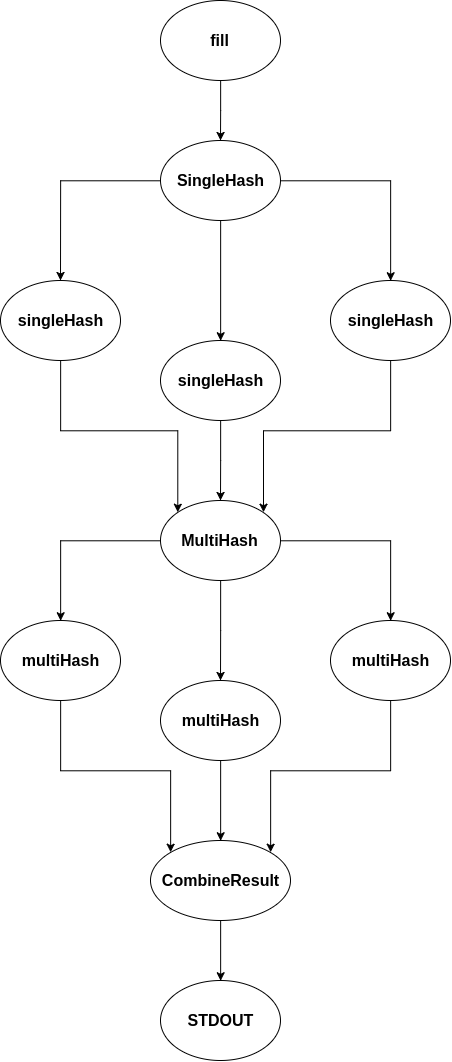
\includegraphics[scale=0.5]{images/codeFlow.png}
\end{center}

\newpage

\paragraph{Листинг кода}

\begin{lstlisting}
package main

import (
	"sync"
	"sort"
	"strings"
	"fmt"
	"strconv"
)

const (
	Th   = 6
	Base = 10
	sliceLen = 10
)

func ExecutePipeline(jobs ...job) {
	channels := make([]chan interface{}, 0)
	for i := 0; i < len(jobs)+1; i++ {
		channels = append(channels, make(chan interface{}, MaxInputDataLen))
	}
	for i, j := range jobs {
		go func(jb job, in, out chan interface{}) {
			jb(in, out)
			close(out)
		}(j, channels[i], channels[i+1])
	}
	fmt.Println(<-channels[len(jobs)])
}

var m sync.Mutex

func singleHash(out chan interface{}, data string) {
	ch := make(chan string)
	go func(ch chan string) {
		ch <- DataSignerCrc32(<-ch)
	}(ch)
	ch <- data
	m.Lock()
	md5 := DataSignerMd5(data)
	m.Unlock()
	crc32md5 := DataSignerCrc32(md5)
	crc32 := <-ch
	out <- crc32 + "~" + crc32md5
}

func SingleHash(in, out chan interface{}) {
	var wg sync.WaitGroup
	for val := range in {
		data := strconv.FormatInt(int64(val.(int)), Base)
		wg.Add(1)
		go func() {
			defer wg.Done()
			singleHash(out, data)
		}()
	}
	wg.Wait()
}

func multiHash(out chan interface{}, data string) {
	var chs [Th]chan string
	var resultHash string
	for i := 0; i < Th; i++ {
		chs[i] = make(chan string)
		go func(ch chan string, i int) {
			ch <- DataSignerCrc32(strconv.FormatInt(int64(i), Base) + data)
		}(chs[i], i)
	}
	for i := 0; i < Th; i++ {
		resultHash += <-chs[i]
	}
	out <- resultHash
}

func MultiHash(in, out chan interface{}) {
	var wg sync.WaitGroup
	for i := range in {
		data := i.(string)
		wg.Add(1)
		go func() {
			defer wg.Done()
			multiHash(out, data)
		}()
	}
	wg.Wait()
}

func CombineResults(in, out chan interface{}) {
	result := make([]string, 0)
	for val := range in {
		result = append(result, val.(string))
	}
	sort.Strings(result)
	out <- strings.Join(result[:], "_")
}

func fib() func() int {
	a, b := 0, 1
	var tmp int
	return func() int {
		tmp, a, b = a, b, a + b
		return tmp
	}
}

func fill(in, out chan interface{}) {
	f := fib()
	for i := 0; i < sliceLen; i++ {
		out <- f()
	}
}
\end{lstlisting}

\newpage

\begin{flushleft}
	\begin{tikzpicture}
	\begin{axis}[
	x=0.012cm,
	title={Работа конвеера при различном количестве входных данных (gobench)},
	xlabel={количество данных},
	ylabel={время $t(ns)$},
	xmin=5, xmax=1300,
	ymin=0, ymax=20000000000,
	legend pos=north west,
	ymajorgrids=true,
	grid style=dashed,
	]
	
	\addplot[
	color=blue,
	mark=star,
	]
	coordinates {
		(5,2051129323)(10,2101912262)(20,2203757776)(40,2407430935)(80,2814972687)(160,3628018451)(320,5260973211)(640,8516648833)(1280,15041182618)
	};
	
	\end{axis}
	\end{tikzpicture}
\end{flushleft}

\paragraph{Тестовые данные}\\

Время работы в секундах (s):\\
\begin{tabular}{l*{9}{c}r}
	Алгоритм & 5 & 10 & 20 & 40 & 80 & 160 & 320 & 640 & 1280 \\
	\hline
	Конвеер & 2.05 & 2.10 & 2.20 & 2.41 & 2.82 & 3.63 & 5.26 & 8.52 & 15.04 \\
\end{tabular}

\newpage

\paragraph{Вывод}

Данная лабораторная работа заключалась в том, чтобы реализовать концепцию конвеера для обработки сложной задачи наиболее эффективно. Если, расмотренную конкрентно в этом документе программу, запускать синхронно для 7 элементов, то это занимает примерно 57 секунд. Сравнив с 15-ю для 1280 элементов, можно утверждать, что цель максимально оптимизировать работу программы была достигнута. Так же данная концепция довольно часто встречается в реальных задачах, где необходимо делать обработчики задач, чтобы максимально эффектно распределять нагрузку на ОС.

\paragraph{Заключение}

В ходе работы была описана и реализована задача конвеера, а именно программа, считающая подпись для слайса данных, и был проведен сравнительный анализ временной эффективности.

\backmatter %% Здесь заканчивается нумерованная часть документа и начинаются ссылки и
            %% заключение

\appendix   % Тут идут приложения

\end{document}

%%% Local Variables:
%%% mode: latex
%%% TeX-master: t
%%% End: